\section{Профилирование}

Профилирование проводилось с помощью утилиты \verb|perf|.

\linespace

Профилировались утилиты \verb|ps-scanner-1| и \verb|ps-scanner-2|. Была собрана информация о (\%) загруженности CPU, функциях программ в пользовательском пространстве и функциях ядра.\\
С помощью \verb|perf record| была собрана данная статистика и сохранена в директории \verb|./profiling/ver1/perf.data| для \verb|ps-scanner-1| и \verb|./profiling/ver2/perf.data| для \verb|ps-scanner-2|.

\linespace

Оба сборщика статистик запускались при следующем тесте: отправлялись 10000 пакетов, 1000 пакетов и затем снова 10000 пакетов с сообщением \verb|"Hello"|.

\vspace{-0.8cm}
\begin{center}
    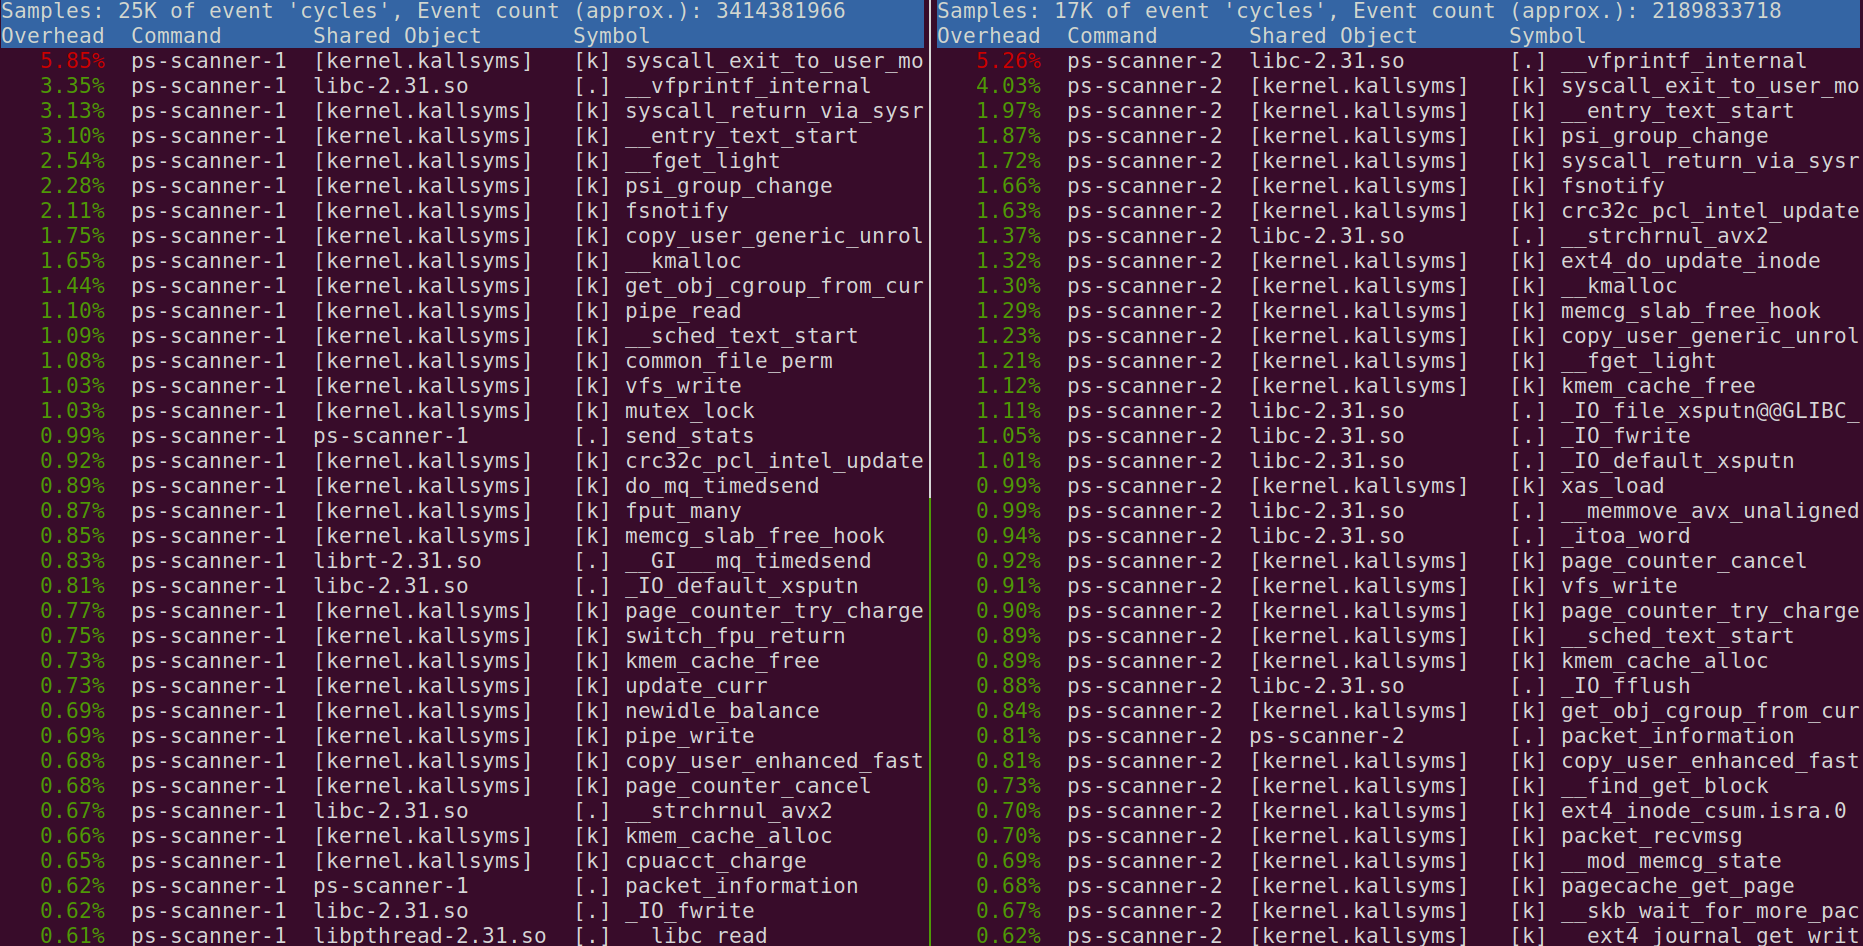
\includegraphics[scale=0.28]{../assets/perf.png}
\end{center}
\vspace{-0.5cm}

На данном рисунке продемонстрированы отчёты утилиты \verb|perf|. Слева -- отчёт утилиты \verb|ps-scanner-1|, справа -- отчёт утилиты \verb|ps-scanner-2|.

\newpage

\subsubsection*{Выводы}

Из данных отчётов можно заметить, что эффективнее процессорное время расходует вторая реализация, которая сразу суммирует статистику. То есть \verb|ps-scanner-2| работает лучше, чем \verb|ps-scanner-1|.\\
Также стоит отметить, что \verb|ps-scanner-2| обрабатывает пакеты быстрее, чем \verb|ps-scanner-1|.
